\chapter{System Architecture}

The VoiceScore system consists of a highly specialized, multi-tier pipeline designed to convert raw vocal signals into detailed, frame-aligned phonetic diagnostic feedback. This chapter details the core architectural components, from initial signal processing to the generation of Goodness of Pronunciation (GoP) scores.

\section{Technical System Flow}
The architecture can be conceptually divided into the Audio Pipeline, the Contrastive CTC Embedding Space, and the Diagnostic Scorer. The flow of data through these components is illustrated conceptually below:

\begin{enumerate}
    \item \textbf{Raw Audio Processing:} Raw 16kHz audio undergoes Fast Fourier Transform (FFT) spectral subtraction to filter out static background noise. A Voice Activity Detector (VAD) trims silence and pads the audio to isolate the active speech segment.
    \item \textbf{Feature Extraction:} The cleaned audio is passed into the Wav2Vec2 base encoder, which outputs contextualized 768-dimensional acoustic frame vectors.
    \item \textbf{Acoustic Projection:} A linear projection layer compresses the 768-dimensional frames into a 256-dimensional space, followed by L2 normalization.
    \item \textbf{Phoneme Embeddings:} The target phoneme vocabulary ($V$) is represented by a learnable embedding matrix ($V \times 256$), which is also L2 normalized.
    \item \textbf{Cosine Similarity Logits:} Matrix multiplication between the normalized audio frames and the normalized phoneme embeddings generates a cosine similarity matrix, which is scaled by a learnable temperature parameter to produce the final logits.
    \item \textbf{Forced Alignment \& Scoring:} The logits are passed through a Softmax layer. A CTC forced aligner maps the probabilities to the target text, generating precise GoP scores for each phoneme.
\end{enumerate}

\begin{figure}[h]
    \centering
    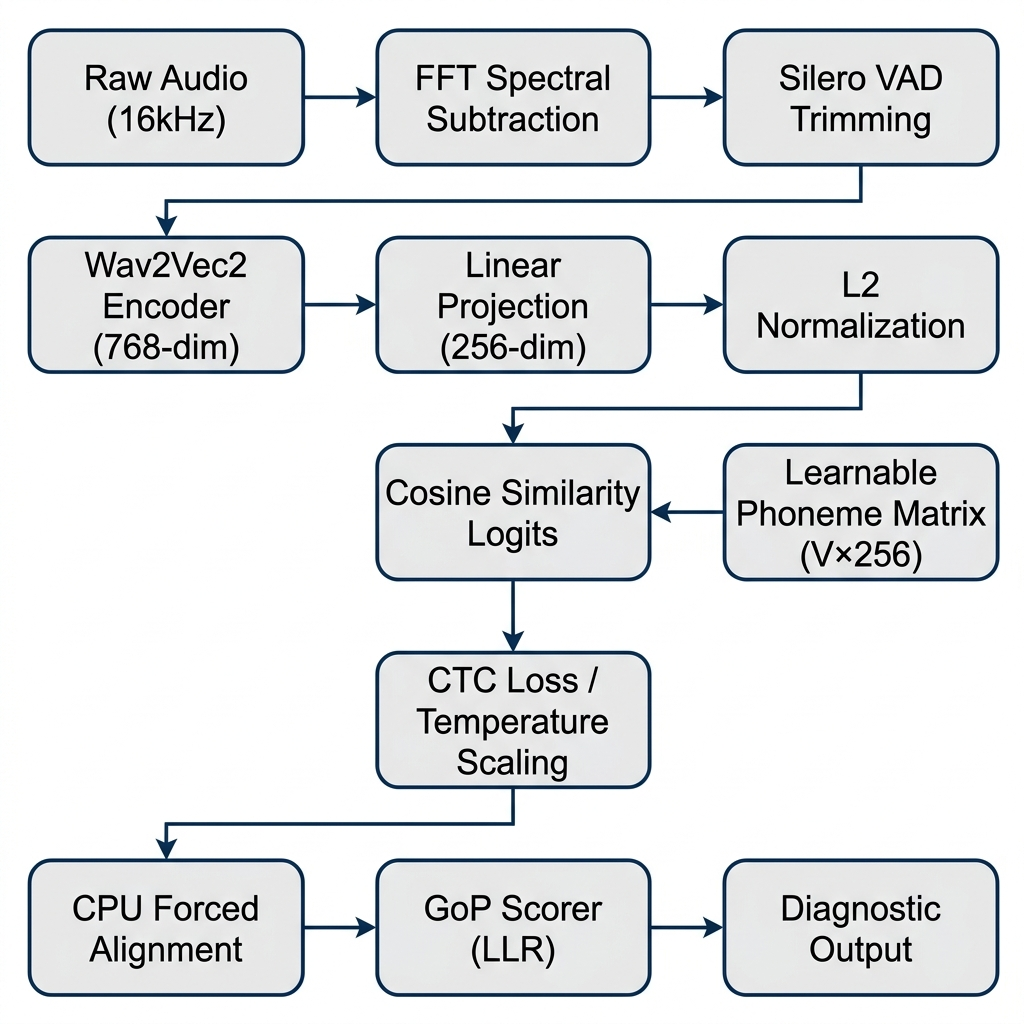
\includegraphics[width=\textwidth]{../docs/asr_architecture.png}
    \caption{Detailed ASR Pipeline Flowchart}
    \label{fig:asr_architecture}
\end{figure}

\section{Evolution: Original Architecture (Standard CTC)}
Before the implementation of the Contrastive CTC embedding space, the original baseline architecture employed a standard CTC classification head. In this early iteration, the 768-dimensional contextualized acoustic frames from the Wav2Vec2 encoder were projected directly into a linear classification layer with an output dimension equal to the vocabulary size (65 phonetic tokens). The model then applied a standard Softmax layer to generate probabilities over the vocabulary. 

While this architecture successfully learned to transcribe clear speech, it suffered from severe instability when calculating Goodness of Pronunciation (GoP). Standard CTC classifiers are highly susceptible to "peaky" distributions—outputting extreme confidence (e.g., 99.9\%) for a few milliseconds and predicting the blank token everywhere else. This peakiness made continuous frame-level scoring erratic, as the acoustic probability of a phoneme would artificially plummet to zero during the sustained articulation of the sound. This fundamental limitation necessitated the architectural shift toward the shared cosine metric space described in the following section, which produces significantly smoother and more robust temporal alignments.

\section{Contrastive Audio-Phoneme Embedding Space}
A standard CTC implementation projects the final encoder states directly into a classification layer with dimensions equal to the vocabulary size. VoiceScore departs from this standard by implementing a Contrastive CTC head.

Instead of direct classification, the model maps both the acoustic frame vectors ($T \times 768$) and the phoneme target vectors ($V \times 256$) into a shared 256-dimensional metric space. Both representations undergo L2 normalization. The likelihood of a phoneme at a given time step is then determined by the cosine similarity between the acoustic vector and the phoneme embedding.

This approach offers two major advantages:
\begin{itemize}
    \item \textbf{Robustness to Variance:} By operating in a normalized metric space, the model focuses on the directional alignment of features rather than their magnitude, making it inherently more robust to volume variations and background noise.
    \item \textbf{Learnable Clustering:} The learnable phoneme embedding matrix allows the model to naturally cluster acoustically similar sounds (e.g., grouping various nasal consonants or retroflex stops together in the 256D space), leading to smoother probability distributions.
\end{itemize}

\section{Schwa Down-Weighting (Anti-Collapse)}
One of the unique challenges of modeling Indian English is the extreme prevalence of the schwa sound (`/ə/`). In many regional accents, the schwa is inserted as an epenthetic vowel to break up complex consonant clusters, making it highly frequent (representing roughly 30\% of all spoken vowels in the dataset).

During early training sessions, this frequency led to representation collapse, where the model would lazily predict the schwa token for any ambiguous acoustic frame, artificially lowering the loss without learning the underlying phonetic nuances.

To combat this, VoiceScore implements a custom Schwa Down-weighting mechanism. We penalize the log-probabilities of highly frequent phonemes during the forward pass by applying an additive weight before the CTC loss calculation:
\begin{equation}
    \log P(\text{adjusted}) = \log P(\text{raw}) + \log(0.3)
\end{equation}
This penalty forces the model to rely on definitive acoustic evidence before committing to a schwa prediction, effectively preventing representation collapse and ensuring high precision across the entire phoneme inventory.

\section{CPU Forced Alignment Safety Net}
To generate phoneme-level scores, the system must perform forced alignment between the predicted logits and the expected target transcription. We utilize \texttt{torchaudio.functional.forced\_align}. However, early in development, ABI CUDA compiler conflicts caused C++ segmentation faults inside the Torchaudio binary when executed on GPUs, particularly within Docker containers.

To guarantee system stability, the forced alignment process is strictly pinned to the CPU. Furthermore, a strict pre-validation safety net was implemented:
\begin{itemize}
    \item The target length $L$ must be less than or equal to the frame length $T$ ($T \ge L$).
    \item The target sequence must not be empty ($L > 0$).
    \item If any of these boundary checks fail, the system elegantly falls back to a linear frame-to-phone time allocator, preventing fatal crashes during runtime.
\end{itemize}
